\documentclass[russian,aspectratio=169,14pt]{beamer}

\usetheme{ShipilevRH}

\title{Работа с файлами}
\subtitle{NIO. Получение ресурсов}
\author{Валерий Алексеевич Овчинников}
\institute{valery.ovchinnikov@phystech.edu}

\begin{document}

\maketitle



\section{Доступ к ресурсам}

\begin{frame}
	\frametitle{Что такое?}
    \begin{center}
	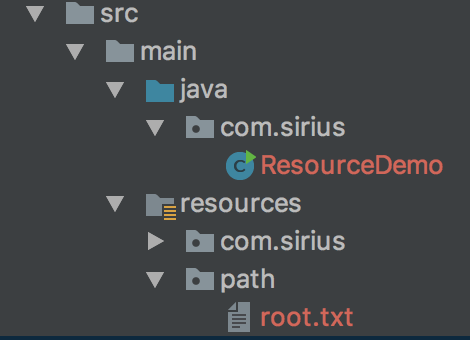
\includegraphics[height=0.75\textheight]{resources.png}
	\end{center}
\end{frame}

\begin{frame}
	\frametitle{Где применяется}
	\begin{itemize}
		\item В JEE контейнерах
		\item В многочисленных фреймворках типа Spring
		\item В собственном коде для конфигурации системы
	\end{itemize}
\end{frame}

\begin{frame}
	\frametitle{Расположение}
	Java ищет ресурсы в окружении исполняемого кода:
	\vfill
	\begin{itemize}
		\item Внутри всех jar-файлов в classpath
		\item Рядом с *.class файлами в classpath
	\end{itemize}
\end{frame}

\begin{frame}[fragile]
	\frametitle{Пути к ресурсам}
	Абсолютный (относительно classpath):
	\begin{listjava}
	"/path/to/resource"
	\end{listjava}
	Относительный (завсист от класса, из которого ищут):
	\begin{listjava}
	"path/to/resource"
	\end{listjava}
\end{frame}

\begin{frame}[fragile]
	\frametitle{Примеры. Class}
	1 и 3 эквивалентны\\
	2 и 4 эквивалентны
	\begin{listjava}
// resolved into $classpath/path/to/resource
URL r = com.sirius.Resource.class.getResource("/path/to/resource");
// resolved into $classpath/com/sirius/path/to/resource
URL r = com.sirius.Resource.class.getResource("path/to/resource");

// resolved into $classpath/path/to/resource
URL r = this.getClass().getResource("/path/to/resource");
// resolved into $classpath/com/sirius/path/to/resource
URL r = this.getClass().getResource("path/to/resource");
	\end{listjava}
\end{frame}

\begin{frame}[fragile]
	\frametitle{Примеры. ClassLoader}
	Только относительные пути!\\
	Всегда относительно classpath
	\begin{listjava}
// resolved into $classpath/path/to/resource
URL r = Thread.currentThread().getContextClassLoader()
             .getResource("path/to/resource");
	\end{listjava}
\end{frame}

\begin{frame}[fragile]
	\frametitle{Примеры. InputStream}
	\begin{listjava}
InputStream is = Resource.class
                   .getResourceAsStream("/path/to/resource");
InputStream is = Resource.class
                   .getResourceAsStream("path/to/resource");
InputStream is = Thread.currentThread().getContextClassLoader()
                   .getResourceAsStream("path/to/resource");
	\end{listjava}
\end{frame}





\section{File NIO}

\begin{frame}
	\frametitle{New IO}
	Было: \textit{Input/OutputStream, ByteStream, CharacterStream}\\
	Стало: \textit{Channels, Buffers}
	\vfill
	Информация копируются из каналов в буферы при чтении и из буферов в каналы при записи
\end{frame}

\begin{frame}
	\frametitle{New IO}
	Появились неблокирующие (non-blocking) вызовы\\
	Появились Selectors
	\vfill
	Теперь можно обрабатывать одновременно несколько каналов с данными в одном потоке (мультиплексирование)
\end{frame}

\begin{frame}
	\frametitle{Основные типы каналов}
	\begin{itemize}
		\item FileChannel
		\item DatagramChannel
		\item SocketChannel
		\item ServerSocketChannel
	\end{itemize}
\end{frame}

\begin{frame}
	\frametitle{Основные буферов}
	\begin{itemize}
		\item ByteBuffer
		\item CharBuffer
		\item DoubleBuffer
		\item FloatBuffer
		\item IntBuffer
		\item LongBuffer
		\item ShortBuffer
	\end{itemize}
\end{frame}

\begin{frame}
	\frametitle{FileChannel}
	\begin{itemize}
		\item FileStream.getChannel()
		\item RandomAccessFile.getChannel()
		\item FileChannel.open(path)
	\end{itemize}
\end{frame}


\begin{frame}
	\frametitle{FileChannel}
	\begin{itemize}
		\item read(buffer)
		\item write(buffer)
		\pause
		\item size()
		\item position($[$position$]$)
		\item truncate(size)
		\pause
		\item close()
		\item force(boolean flushMetaData)
	\end{itemize}
\end{frame}


\begin{frame}[fragile]
	\frametitle{Пример. Чтение}
	\begin{listjava}
ByteBuffer buf = ByteBuffer.allocate(48);
int bytesRead = inChannel.read(buf);
while (bytesRead != -1) {
    // NOTICE!!
    buf.flip();
            
    while (buf.hasRemaining()) {
        System.out.print((char) buf.get());
    }
            
    buf.clear(); // or buf.compact()
    bytesRead = inChannel.read(buf);
}
	\end{listjava}
\end{frame}

\begin{frame}[fragile]
	\frametitle{Пример. Запись}
	\begin{listjava}
ByteBuffer buf = ByteBuffer.allocate(bytes.length);
buf.put(bytes);
        
buf.flip();
        
while (buf.hasRemaining()) {
    outChannel.write(buf);
}
buf.clear();
	\end{listjava}
\end{frame}

\begin{frame}[fragile]
	\frametitle{Пример. Позиционирование}
	\begin{listjava}
// write
outChannel.position(writeOffset);
while (buf.hasRemaining()) {
    outChannel.write(buf);
}

//read
inChannel.position(readOffest);
int bytesRead = inChannel.read(buf);
	\end{listjava}
\end{frame}

\begin{frame}
	\frametitle{Ужасы ByteBuffer}
	У ByteBuffer есть 3 параметра:
	\begin{itemize}
		\item Capacity (постоянное значение, общий размер буфера)
		\item Position (зависит от режима: конец записи/начало чтения)
		\item Limit (зависит от режима: capacity/конец чтения)
	\end{itemize}
\end{frame}

\begin{frame}
	\frametitle{Ужасы ByteBuffer}
	\begin{minipage}{0.55\textwidth}
	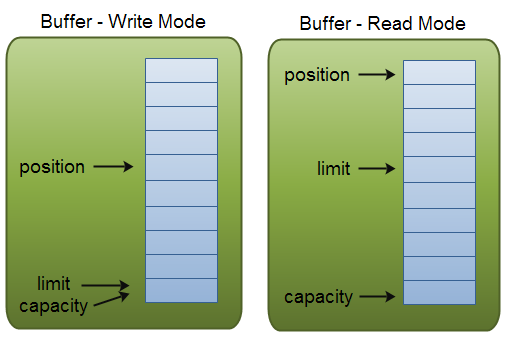
\includegraphics[height=0.75\textheight]{byte_buffer.png}
	\end{minipage}
	\hfill
	\begin{minipage}{0.2\textwidth}
	\begin{itemize}
		\item Capacity
		\item Position
		\item Limit
	\end{itemize}
	\end{minipage}
\end{frame}

\begin{frame}[fragile]
	\frametitle{Ужасы ByteBuffer}
	rewind -- вернет position в значение 0, можно будет снова читать сначала
	\begin{listjava}
buf.get(); // a
buf.get(); // b
buf.rewind();
buf.get(); // a
	\end{listjava}
\end{frame}

\begin{frame}[fragile]
	\frametitle{Ужасы ByteBuffer}
	mark -- запомнит текущую position
	reset --  выставит помеченый position
	\begin{listjava}
buf.mark(); // position = 3
buf.get(); // position = 4
buf.get(); // position = 5
buf.reset(); // position = 3
	\end{listjava}
\end{frame}

\begin{frame}[fragile]
	\frametitle{Ужасы ByteBuffer}
	clear -- переводит в режим записи в буфер, position = 0, limit = capacity
	compact -- переводит в режим записи в буфер, непрочитанное копирует в начало, position = n, limit = capacity
	\begin{listjava}
buf.get();
buf.compact();
	\end{listjava}
\end{frame}

\begin{frame}[fragile]
	\frametitle{Path}
	Замена класса java.io.File
	\begin{itemize}
		\item get
		\item normalize
		\item toAbsolutePath
	\end{itemize}
	\begin{listjava}
Path path = Paths.get("c:\\path\\to\\myfile.txt");
Path path = Paths.get("/path/to/myfile.txt");
Path path = Paths.get("/path", "to", "myfile.txt");
// relative to dir from which code is executed
Path path = Paths.get("relative/path/to/myfile.txt");
	\end{listjava}
\end{frame}

\begin{frame}
	\frametitle{Files}
	\begin{itemize}
		\item exists
		\item createDirectory
		\item copy
		\item move
		\item delete
		\item walkFileTree
	\end{itemize}
\end{frame}

\begin{frame}[fragile]
	\frametitle{Files}
	\begin{listjava}
Path from;
Path to;	
if (Files.exists(from)) {
    Files.delete(from);
} else {
    Files.createDirectory(newDirectory);
}
Files.copy(from, to);        
Files.move(from, to, StandardCopyOption.REPLACE_EXISTING);
	\end{listjava}
\end{frame}

\begin{frame}[fragile]
	\frametitle{Channel-to-Channel File Copy}
	\begin{listjava}
from.transferTo(0, from.size(), to);
to.transferFrom(from, 0, from.size());
	\end{listjava}
\end{frame}

\begin{frame}[fragile]
	\frametitle{AsynchronousFileChannel}
	\begin{listjava}
Future<Integer> future = fileChannel.read(buf, position);
fileChannel.read(buffer, position, attachement, 
        new CompletionHandler<Integer, ByteBuffer>() {
            @Override
            public void completed(Integer result, 
                 ByteBuffer attachment) {}
        
            @Override
            public void failed(Throwable exc, 
                 ByteBuffer attachment) {}
        });
	\end{listjava}
\end{frame}

\questions

\end{document}
